\section{Linearized equations}\label{linear_problem}
To compute explicit solutions to the linear problem, 
we consider radially-localized axisymmetric disturbances of the form  
\begin{align}
  \delta X (r, z) = \delta X_1(r,z)\exp{(\ii k_x r)},
\end{align} 
%and similarly for $\dd P$ and $\dd\bm{v}$. 
where $k_x$ is a real wavenumber such that $|k_xr|\gg 1$, and the 
amplitude $\dd X_1(r,z)$ is 
a slowly-varying function of $r$. Then 
$\p_r\to i k_x$ when acting on the above primitive perturbations, and we may
neglect curvature terms. We take  
$k_x>0$ without loss of generality. Hereafter, we drop the subscript 1
on the amplitudes. 
%The frequency $\sigma = \omega +
%\ii s$ is generally complex, with $\omega$ being the real frequency
%and $s$ is the real growth rate. 

Introducing 
\begin{align}
  W \equiv \frac{\dd\rho}{\rho}, \quad Q \equiv \frac{\dd P}{\rho},
\end{align}
the linearized equations for 
vertically isothermal dusty gas with the pressure
equation in place of the dust-fraction
(Eq. \ref{masseq}---\ref{momeq}, Eq. \ref{eff_energy}) are then:    

\begin{align}
  \ii\sigma W &= \ii k_x \dd v_r + \dd v_z^\prime +
  \dd v_r \p_r\ln{\rho} + \dd v_z\p_z\ln{\rho},\label{lin_mass}\\
  -\ii\sigma\dd v_r  &= 2\Omega\dd v_\phi 
% +  \delta\bm{F}\cdot\hat{\bm{r}}
- W F_r - \ii k_x Q - \ii k_x\dd\psi,\label{lin_xmom}\\
  \ii\sigma\dd v_\phi &= \frac{\kappa^2}{2\Omega}\dd v_r + \frac{\p
    v_\phi}{\p z}\dd v_z, \label{lin_ymom}\\
  -\ii\sigma\dd v_z &= - W F_z - \left[Q^\prime + Q
    \left(\ln{\rho}\right)^\prime\right] - \dd\psi^\prime  %\delta\bm{F}\cdot\hat{\bm{z}} 
,\label{lin_zmom}\\
  \ii\sigma Q &= \frac{P}{\rho}\left(\ii k_x \dd v_r + \dd
               v_z^\prime\right) + \frac{1}{\rho}\left(\dd v_r\p_rP + \dd v_z \p_zP\right)\notag\\
                &\phantom{=}-\frac{P}{\rho} \dd v_r\p_r
               \ln{c_s^2} %, \label{lin_energy} 
%+ \dd v_z \p_z\ln{c_s^2}\right),\label{lin_energy} 
               - \frac{\dd\mathcal{C}}{\rho},\label{lin_energy}\\
\dd\psi^{\prime\prime}  &= 4\pi G \rho W + k_x^2\dd\psi, \label{lin_sg}
\end{align}  
where $^\prime \equiv \p_z$ and recall $\bm{F} \equiv -\nabla
P/\rho$. Here we restore self-gravity temporarily for SGI in the next
section. The linearized dust-duffusion function 
$\dd\mathcal{C}$ is given in  Appendix \ref{lin_dust}. 
% and $\dd\bm{F}$ is the linearized pressure
%force, given in Appendix \ref{lin_press}. 
%Note that we have assumed a temperature profile that only depends on $r$.   

%; and 
%\begin{align}
%  \delta \bm{F} \equiv \frac{\dd\rho}{\rho^2}\nabla P -
%  \frac{1}{\rho}\nabla\dd P, 
%\end{align}
%$\dd\mathcal{C}$ is the linearized dust-duffusion function, given in
%Appendix \ref{lin_dust}. We consider stopping times appropriate for
%small grains in the Epstein regime. Note that for the axisymmetric
%problem, $\dd\bm{F}$ is purely meridional. 

Eq. \ref{lin_mass}---\ref{lin_sg} is a set of ordinary
differntial equations in $z$. All coefficients and amplitudes are
evaluated at a fiducial radius $r=r_0$, but their full $z$-dependence
is retained. We next discuss solutions to these equations.  We first
show that the above equations yield the secular
gravitational instability and streaming instability in the strong
drag regime in \S\ref{sgi} and \S\ref{si}, respectively. We then
consider 3D, stratified disks in \S\ref{results} to study the dusty
vertical shear instability.

%for a
%razor-thin, self-gravitating disk in \S\ref{sgi}; and for 3D
%non-self-gravitating, unstratified and stratified disks 
%in \S\ref{si} and \S\ref{results}, respectively.   
 
 % Numerical solutions are generally required for the 
%vertically-stratified problem. 

%\section{Connection to previous results}

\subsection{Secular gravitational instability}\label{sgi}
We first consider a razor-thin, self-gravitating disk so that $\rho =
\Sigma\delta(z)$. Here $\delta$ is the Dirac delta function and $\Sigma$ is
the total surface density. Now $\epsilon$ and 
$\tepsilon$ refers to the global dust-to-gas ratio and dust 
fraction, respectively. The background disk is
uniform and we neglect the vertical dimension   
in Eq. \ref{lin_mass}---\ref{lin_energy}. The linearized dust-gas drag
term is then $-\delta\mathcal{C}/\rho = \tstop\tepsilon c_s^2k_x^2
Q$. The thin-disk solution to Eq. \ref{lin_sg} is $\dd\psi(z=0) = -2\pi G
\Sigma W/\left|k_x\right|$.%, where $\Sigma$ is the total surface
%density. 

These simplifications yield the dispersion relation
\begin{align*}
  \left(\ii\sigma - \tstop\tepsilon c_s^2k_x^2\right)\left( 2 \pi G
    \Sigma \left|k_x\right|  - \kappa^2 + \sigma^2 \right) = \ii
  \sigma c_s^2 k_x^2\left(1 - \tepsilon\right). 
\end{align*}
Searching for slowly and purely growing modes, $\sigma = \ii s$ with 
$|s|\ll \kappa$, we find 
\begin{align}  
s = \frac{\tstop\tepsilon c_s^2 k_x^2 \left( 2 \pi \Sigma G
    \left|k_x\right| - \kappa^2\right)}{\kappa^2 -2 \pi \Sigma G
    \left|k_x\right| + c_s^2k_x^2\left(1-\tepsilon\right) }. \label{sgi_disp}
\end{align}
This is secular gravitational instability mediated by strong
dust-gas drag with negligible turbulent dust diffusion 
\citep[][ their Eq. 13 becomes our Eq. \ref{sgi_disp} in this limit
after 
a change of variables]{takahashi14}. A similar effect occurs in viscous
self-gravitating gas disks \citep{gammie96,lin16}. In fact, if we
identify $\nu \equiv \tstop \tepsilon c_s^2$ as a kinematic viscosity,
then Eq. \ref{sgi_disp} is identical to \citeauthor{gammie96}'s Eq. 18. 

This exercise shows that the one-fluid framework, further simplified by
the terminal velocity approximation, is sufficient to capture SGI
in the strong drag limit. 

\subsection{Streaming instability}\label{si}
We now consider 3D disks without self-gravity. We neglect the vertical     
component of the stellar gravity, appropriate for studying regions
near the disk midplane. This  
allows us to Fourier analyze in $z$ to obtain 
an algebraic dispersion relation of the form  
$\sum_{j=0}^{5}c_j(k_x,k_z)\sigma^j = 0$, where $k_z$ is a real
vertical wavenumber. The coefficients $c_j$ can be read 
off Eq. \ref{streaming_dispersion} in  Appendix \ref{compressible_streaming}. 
There we also show that this dispersion relation reduces to that for
the streaming instability (SI) in the limit of incompressible gas and small
$\tstop$ \citep{youdin05a,jacquet11}.   
 
%\subsection{Numerical examples}

%{\bf note: kappa2 accounts for dust effect assuming smallh=0.05}

In Table \ref{si_compare} we solve the full dispersion relation
(Eq. \ref{streaming_dispersion}) numerically for selected cases where
analytic SI growth rates have been verified with particle-gas
numerical simulations \citep[namely][]{youdin07b,bai10b}.  
Following previous works on SI, we use normalized 
wavenumbers $K_{x,z} = \eta r k_{x,z}$ where
\begin{align} 
  \eta \equiv -\frac{1}{2\rhog r\OmK^2}\frac{\p P}{\p r} = 
  \frac{1}{2\left(1-\tepsilon\right)}\frac{F_r}{r\OmK^2}, 
\end{align} 
measures the pressure offset of Keplerian rotation. We fix 
$\eta=0.05c_s/r\OmK$. In this section section we also quote the
particle stopping time $\tau_\mathrm{s}=\tstop/(1-\tepsilon)$.    

The eigenfrequencies obtained from the one-fluid dispersion relation 
are compared that from a full, two-fluid analysis \citep[similar 
to][]{youdin05a, kowalik13}. As expected eigenfrequencies agree better
with decreasing $\taus$ since in that limit the mixture behaves more 
like a single fluid. Most importantly, we find the work done
$\mathcal{W}>0$ in all cases, and hence find growing oscillations. 

%{\bf note: important to use largrangian pressure pert properly}

% We also checked the growth rates $s$ satisfy 
% \begin{align} 
%   s = \frac{\left|\sigma\right|^2\imag\left(\Delta P
%     \Delta\rho^*/\rho\right)}{2\real\left(\sigma\right)\rho\left(\left|\dd
%   v_x\right|^2+\left|\dd
%   v_z\right|^2\right)}, \label{si_check}
% \end{align}
% as implied by Eq. \ref{thermal_instability} and
% Eq. \ref{pdv}. %, or directly from
% %Eq. \ref{streaming_mass}---\ref{streaming_vz}. 
% Interestingly, we find in dust-rich disks with 
% $\epsilon>1$, Eq. \ref{si_check} can be satisified with $\Delta
% P\simeq \ii\dd v_x \p_rP/\sigma$, i.e. the radial pressure gradient
% is responsible for growth. Conversely, for `linB' with $\epsilon
% < 1$, one can approximate $\Delta P \simeq \dd P$ in Eq. \ref{si_check}.
% This
%suggests that for SI in gas-dominated disks, the distinction between
%Eulerian and Lagragian pressure perturbations is unimportant. 
%{\bf but weak growth in this case}
%However
%in that case the gro 

In Table \ref{si_compare} we also calculate the phase difference
between the Lagragian pressure perturbation and density perturbations
as    
\begin{align*} 
\varphi&\equiv \sgn{\left[\real{(\sigma)}\right]}\arg\left(\Delta
  P\Delta\rho^*\right).\notag 
%\notag\\
%       &= \sgn{\left[\real{(\sigma)}\right]}\arg\left(\Delta\rhog^*\Delta\rhod\right).\notag
\end{align*}

(Note that $\Delta P = \delta P + \ii \dd v_x \p_rP/\sigma$, and it is
important to include the global radial pressure gradient here.) Then
$\varphi > 0 $ indicates gas pressure lagging behind total density,
which is true for all the cases. Thus SI is indeed associated with
such a phase lag.




In a future work we will perform a detailed comparison between the
simplified one-fluid and full two-fluid frameworks in calculating SI. 




\begin{figure}
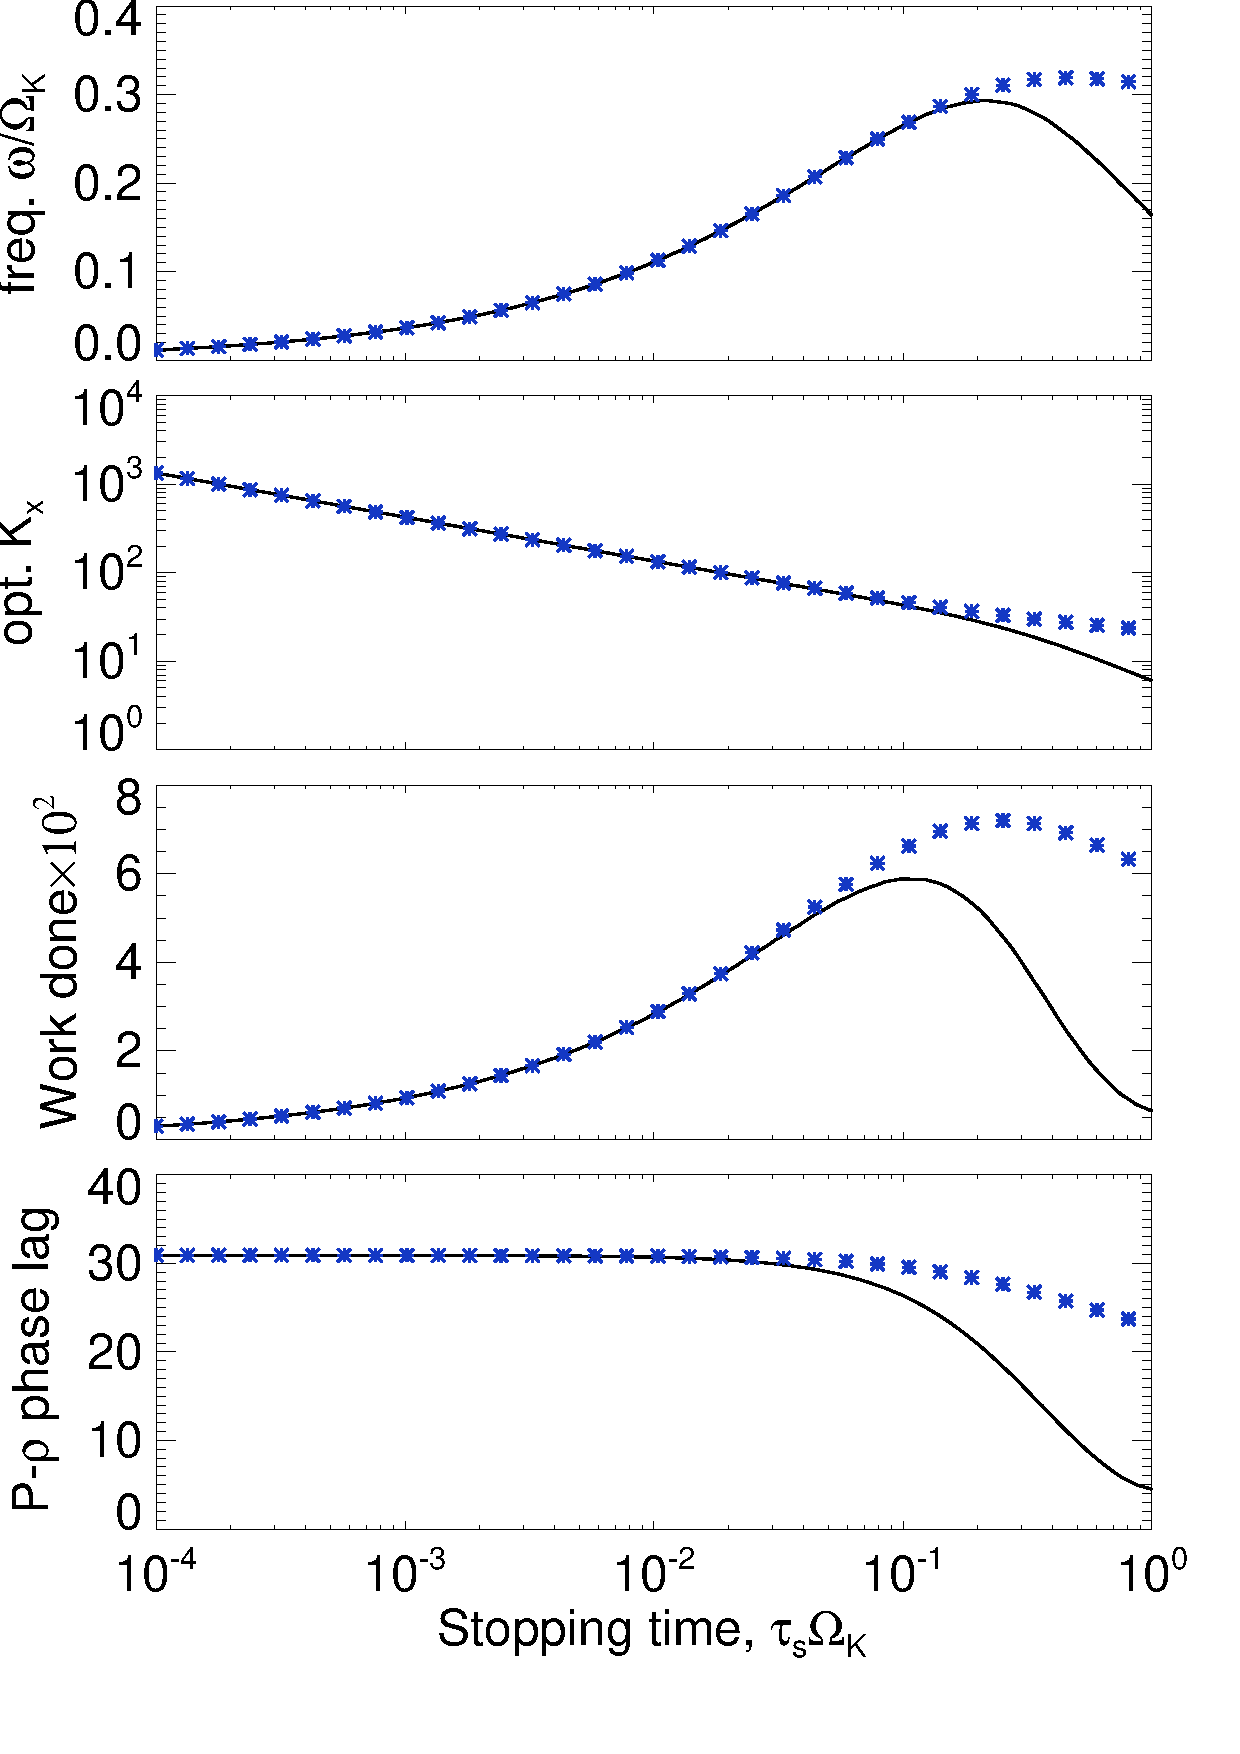
\includegraphics[width=\linewidth]{figures/si_2f_1f_compare}
\caption{{\bf in case the paper isn't long enough} Comparison of the linear
streaming instability obtained from a full two-fluid analysis and the current 
one-fluid framework simplified by the terminal velocity approximation. The vertical
wavenumber is fixed and growth rates are maximized over $K_x$. 
\label{si_compare_full}}
\end{figure}
%"generalized stokes number" would include other problem parameters,
%e.g. wavenumber  


%{\bf suppose large scale pressure grad drops outwards. 
%pert the sys by kicking more dust inwards. gas moves out, into region 
%  of lower pressure in the bg. i.e. create pressure bump at larger
%  radius. it attracts the first dust particles back out, plus some more
%  because bump is larger. (move gas from higher density to lower
%  density produce asymmetric bump/trough.}

% \begin{deluxetable*}{llrrrrrr}
%   \tablecolumns{8}
%   \tablecaption{Selected eigenfrequencies for the streaming
%     instability. \label{si_compare}
%   }
%   \tablehead{
%     \colhead{Mode} & 
%     \colhead{$\tau_\mathrm{s}\OmK$} &
%     \colhead{$\epsilon$} &
%      \colhead{$K_{x,z}$} &
%       \colhead{$\sigma/\OmK$ (two-fluid)} &
%     \colhead{$\sigma/\OmK$ (one-fluid)} &
%     \colhead{$\mathcal{W}$ (arbitrary units)} &
%       \colhead{$\Delta P$ lag}
%   }
% \startdata
%  linA, \cite{youdin07b} &  $0.1$       & 3.0 & 30    & $0.3480 +
%  0.4190\ii$ & $0.3640 + 0.4249\ii$ & $0.90$ & $30\degr$\\ 

% linB, \cite{youdin07b} & $0.1$        &  0.2 & 6 & $-0.4999 +
% 0.0155\ii$&   $-0.4981 + 0.0054\ii$  & $1.54$ & $1.2\degr$ \\

% linC,  \cite{bai10b}  & $10^{-2}$   &  2.0 & 1500&   $0.1049 +
% 0.5981\ii$   &  $0.1338 + 0.6650\ii$  & $0.15$& $11\degr$ \\

% linD, \cite{bai10b} &  $10^{-3}$   &  2.0 & 2000 & $0.3225 + 
% 0.3154\ii$& $0.3219 + 0.3154\ii$ &  $1.28$ & $22\degr$ 
% \enddata
% \end{deluxetable*}


\begin{deluxetable*}{lrrrrrr}
  \tablecolumns{8}
  \tablecaption{Selected modes of the streaming
    instability. \label{si_compare}
  }
%  \tablehead{
%    \colhead{Mode} & 
%    \colhead{$\tau_\mathrm{s}\OmK$} &
%    \colhead{$\epsilon$} &
%     \colhead{$K_{x,z}$} &
%    \colhead{Complex frequency} &
%    \colhead{$\sigma/\OmK$} &
%    \colhead{Work done} &
%    \colhead{$\mathcal{W}/\left|\Delta P\Delta\rho^*/\rho\right|$} &
%    \colhead{Pressure-density lag} &
%    \colhead{$\varphi$} 
%  }
\startdata
\hline\hline
\multicolumn{1}{c}{Mode ($\tau_\mathrm{s}\OmK$, $K_{x,z}, \rhog/\rhod$)} &
\multicolumn{2}{c}{Complex frequency, $\sigma/\OmK$} &
\multicolumn{2}{c}{Work done, $\mathcal{W}/\left|\Delta P\Delta\rho^*/\rho\right|$} &
\multicolumn{2}{c}{Pressure-density lag, $\varphi$} \\
\hline
\multicolumn{1}{c}{} &
 \multicolumn{1}{c}{two-fluid} &
 \multicolumn{1}{c}{one-fluid} &
 \multicolumn{1}{c}{two-fluid} &
 \multicolumn{1}{r}{one-fluid} &
 \multicolumn{1}{c}{two-fluid} &
 \multicolumn{1}{r}{one-fluid} \\
 \hline
% \multicolumn{6}{c}{\textcolor{blue}{linA\tablenotemark{$\dagger$}: $\tau_\mathrm{s}\OmK=0.1$, $K_{x,z}=30$, $\rhog/\rhod = 3$}}\\
% \hline
linA\tablenotemark{$\dagger$} ($0.1, 30, 3$) &
$0.3480 + 0.4190\ii$ & $0.3640 + 0.4249\ii$ & $0.078$ & $0.090$ & $27\degr$ & $30\degr$  \\
% \hline
% \multicolumn{6}{c}{\textcolor{blue}{linB\tablenotemark{$\dagger$}: $\tau_\mathrm{s}\OmK=0.1$, $K_{x,z}=6$, $\rhog/\rhod = 0.2$}} \\
% \hline
linB\tablenotemark{$\dagger$} ($0.1, 6,0.2$) &
$-0.4999 + 0.0155\ii$&   $-0.4981 + 0.0054\ii$ & 0.025   & $0.0054$ & $5.8\degr$  &  $1.2\degr$  \\
% \hline
% \multicolumn{6}{c}{\textcolor{blue}{linC\tablenotemark{$\ddagger$}: $\tau_\mathrm{s}\OmK=10^{-2}$, $K_{x,z}=1500$, $\rhog/\rhod = 2$}} \\
% \hline
linC\tablenotemark{$\ddagger$} ($10^{-2}, 1500, 2$) &
$0.1049 + 0.5981\ii$   &  $0.1338 + 0.6650\ii$ & 0.0076 & $0.013$ & $8.3\degr$ &$11\degr$  \\
% \hline
% \multicolumn{6}{c}{\textcolor{blue}{linD\tablenotemark{$\ddagger$}: $\tau_\mathrm{s}\OmK=10^{-3}$, $K_{x,z}=2000$, $\rhog/\rhod = 2$}} \\
% \hline
linD\tablenotemark{$\ddagger$} ($10^{-3}, 2000, 2$) &
$0.3225 +  0.3154\ii$& $0.3219 + 0.3154\ii$ &  $0.061$ & $0.061$  & $22\degr$ & $22\degr$  
\enddata
\tablenotetext{$\dagger$}{\cite{youdin07b}}
\tablenotetext{$\ddagger$}{\cite{bai10b}}
\end{deluxetable*}

In Fig. \ref{si_compare_fig} we calculate the most unstable SI 
mode as a function of $\taus$ at fixed $K_z=30$ and $\epsilon =3$. We
compare results between the full, two-fluid linear analysis and the
one-fluid framework. We also include an analytic model, described in Appendix 
\ref{si_dust_rich}, based on the one-fluid dispersion relation with 
additional approximations (orange diamonds).

Both results based on the one-fluid framework compares well with the 
full, two-fluid analysis, only breaking down at a relatively large
$\taus\OmK\gtrsim 0.1$. For larger $\taus$ the two-fluid phase
lag drops, along with the growth rate. This suggest that a
non-vanishing phase lag is necessary for instability. However, the
magnitude of the phase lag does not correlate with growth rates. In
fact, $\varphi$ remains finite as $|\sigma|, \taus\to0$ (but
non-zero). This arises because the optimum $K_x\propto \taus^{-1/2}$
diverges (see Appendix \ref{si_dust_rich}).   

In a future work we will perform a more detailed parameter survey to
compare the simplified one-fluid and full two-fluid frameworks in
calculating SI.  

\begin{figure}
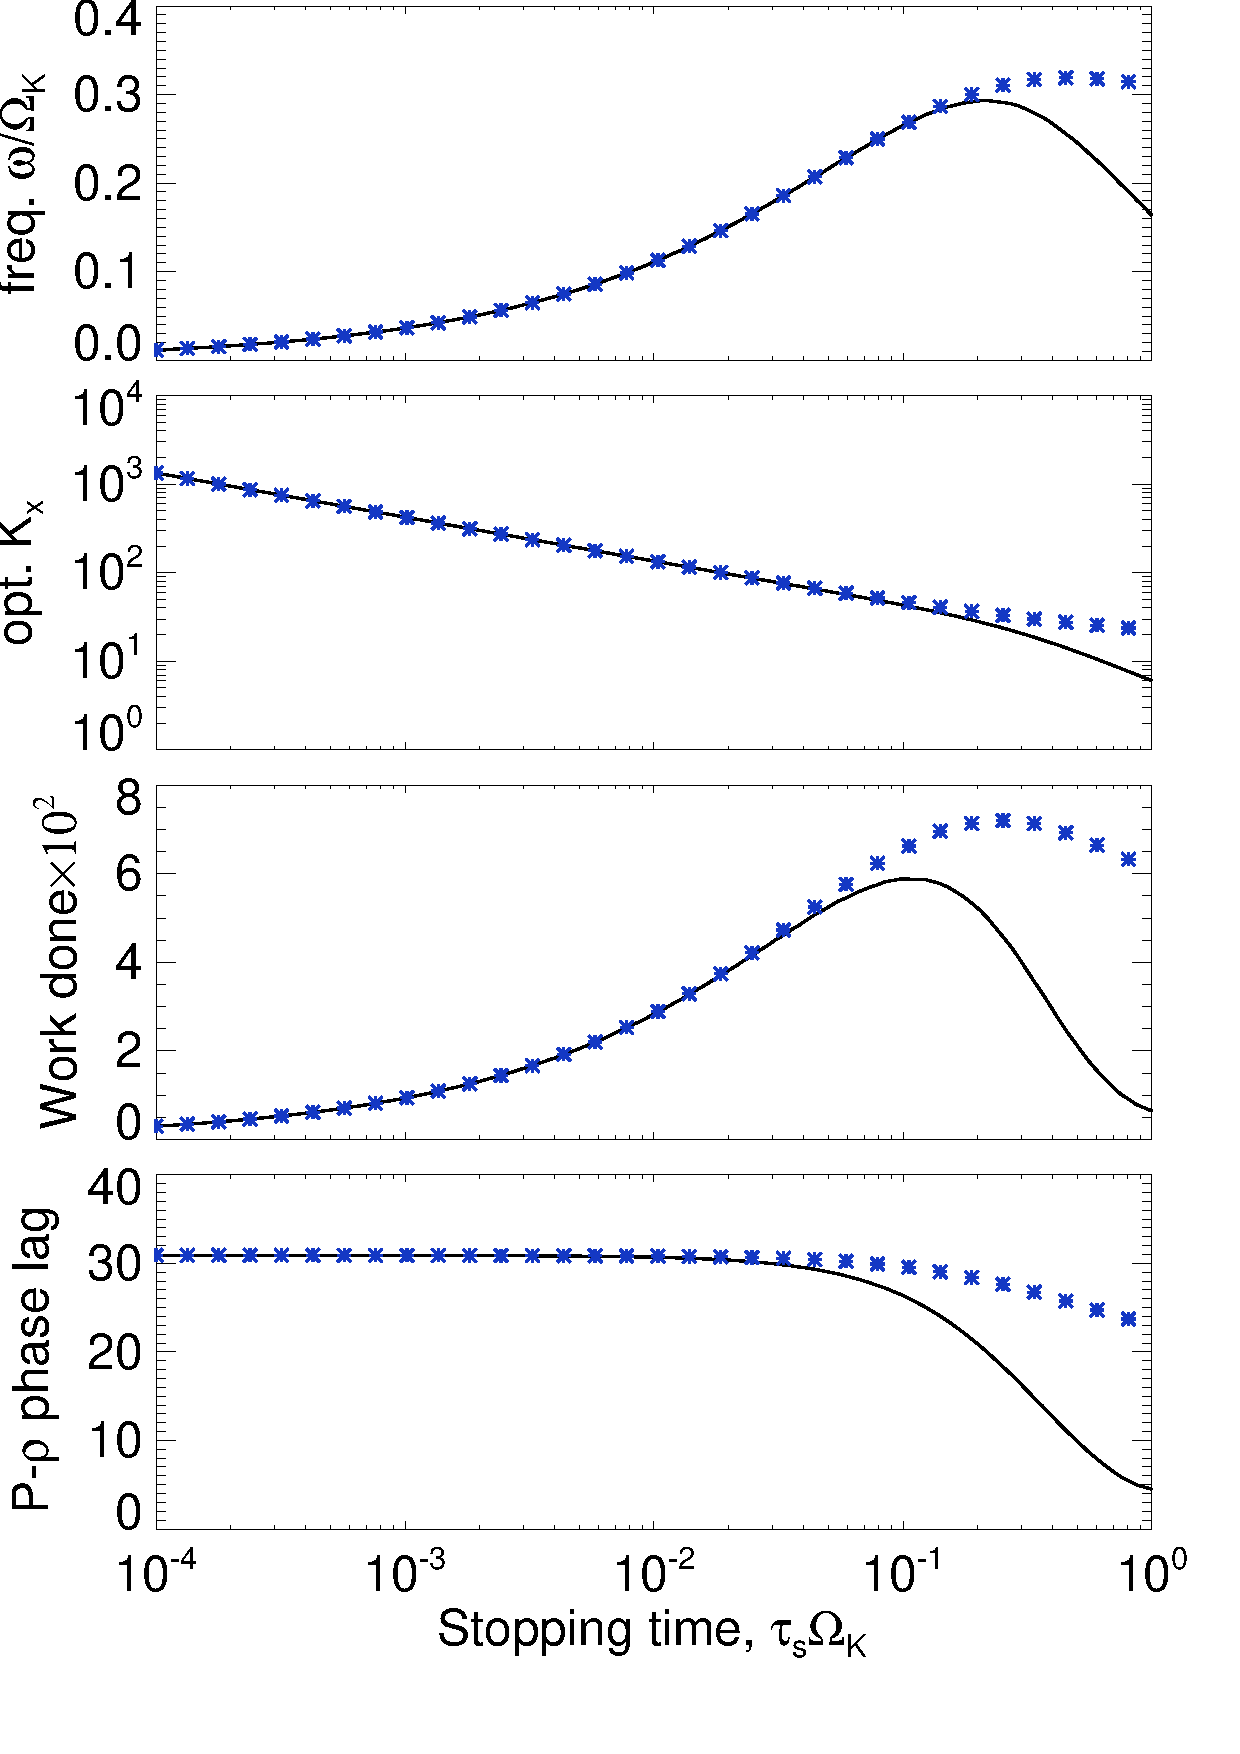
\includegraphics[width=\linewidth]{figures/si_2f_1f_compare}
\caption{Comparison of the linear
streaming instability between a full two-fluid analysis (solid
line), the one-fluid framework simplified by the terminal
velocity approximation (green asterisks) and an analytic solution to
the one-fluid dispersion relation in the dust-rich limit (orange
diamonds, see also Appendix \ref{si_dust_rich}). The vertical 
wavenumber is fixed and growth rates are maximized over $K_x$. 
\label{si_compare_fig}}
\end{figure}






%"generalized stokes number" would include other problem parameters,
%e.g. wavenumber  





% \subsection{Eulerian interpretation}

% We can also consider SI in the Eulerian sense \citep[as
% did][]{jacquet11}. Eq. \ref{thermal_instability} imply SI requires
% \begin{align*}
%   \frac{\imag\left[\delta\mathcal{C}\nabla\cdot\dd\bm{v}^*\right]}{\real(\sigma)}<0. 
% \end{align*}
% The linearized dust diffusion or `cooling' term $\delta\mathcal{C}$
% for this problem is given by Eq. \ref{lin_drag_si}. Thus the
% requirement is 
% \begin{align*}
% \tepsilon |\bm{k}|^2 
%   \frac{\imag\left(\ii \sigma^* QW^*\right)}{\real(\sigma)}
% -k_x F_r\left( 1-2\tepsilon\right) 
%  | W |^2\frac{\imag\left(\sigma^*\right)}{\real(\sigma)} < 0, 
% \end{align*}
% where we have used Eq. \ref{streaming_mass}. 
% For slow growth and/or large $\left|\bm{k}\right|^2$ the second term 
% is small compared to the first. In this case instablity is due to  


%\subsection{Boundary conditions}
%Eq. \ref{lin_mass}---\ref{lin_energy} can be reduced to a set of
%first-order differential equations for $W, Q$ and $\dd v_z$. We can
%see this schematically as follows. Eq. \ref{lin_xmom} and
%\ref{lin_ymom} may be combined to yield 
%\begin{align*}
%  \dd v_r = \dd v_r (W, Q, \dd v_z). 
%\end{align*} 
%We can then take the continuity equation as an equation for $\dd v_z$, 
%\begin{align*}
%\text{Eq. \ref{lin_mass}} \Rightarrow \dd v_z^\prime(z) = \dd
%  v_z^\prime(W,Q,\dd v_z),
%\end{align*}
%and the vertical momentum equation as an equation for $Q$, 
%\begin{align*}
%\text{Eq. \ref{lin_zmom}} \Rightarrow Q^\prime(z) = 
% Q^\prime(W,Q,\dd v_z). 
%\end{align*}

%Now, for finite dust-gas coupling, $\tstop\neq0$, inspection of $\dd C$
%(Appendix \ref{lin_dust}) shows that it involves $W^\prime$ (assuming
%$\tepsilon < 1$). Then Eq. \ref{lin_energy} may be taken as a
%differential equation for $W$. However, for perfectly coupled dust,
%$\tstop =\dd\mathcal{C}= 0$. In that case Eq. \ref{lin_energy} gives an algebraic
%relation between $W$, $Q$ and $\dd v_z$. That is,
%\begin{align*}
%\text{Eq. \ref{lin_energy}}\Rightarrow \begin{cases}
%  W^\prime(z) = W^\prime(W, Q, \dd v_z) & \text{if } \tstop \neq 0, \\
%  W           (z) = W(Q, \dd v_z) & \text{if }\tstop = 0.
%\end{cases}
%\end{align*} 

%This means that for the perfectly coupled problem, we have a pair of
%ODEs for $Q$ and $\dd v_z$, and 
%When
%$\tstop\neq0$, we require three boundary conditions. {\bf WHAT?? Why odd
%  number of BCs? Shouldn't we have even number of BCs? We have
%two boundaries? I've only seen problems like this involving even
%number of BCs.} In this case we impose $\dd v_z =0$ at $z=\pm
%z_\mathrm{max}$, and classify modes according to their symmetry about
%the midplane: `even' modes with $\dd v_z^\prime(0) = 0$, and `odd' 
%modes with $\dd v_z(0)=0$.       

